Nesta secção iremos discutir os resultados obtidos pelos modelos no capítulo \ref{cap:exper}. O principal foco é consolidar um resumo de cada teste nos conjuntos de dados e analisar se o modelo final otimizado pelo Optuna teve um aumento de performance em relação aos modelos com os hiperparâmetros \textit{Default}.

Nos testes iniciais a performance dos modelos foi variável, em alguns testes o XGBoost se destacou, outros o CatBoost e outros o LightGBM. Em termos de custo computacional, o CatBoost é o mais custoso enquanto que o LightGBM foi o teve a melhor performance do ponto de vista de execução computacional.

Esses resultados eram de fato esperados, conforme foi abordado no capítulo \ref{chapter:algoritmos-boosting}. O fato do CatBoost precisar lidar com as variáveis categóricas e a simetria da árvore o torna mais lento, enquanto o LightGBM foi criado justamente para ser mais rápido.

Nos primeiros testes não foi possível identificar o impacto do $LR$ e do $Reg_L$ diretamente na performance dos modelos, o hiperparâmetro que ficou mais em evidência foi o $MD$. Na maioria dos casos, o seu aumento ocasionou um maior tempo de execução, o que de fato era esperado pois esse hiperparâmetro representa o crescimento máximo da profundidade da árvore.

Os principais resultados desse estudo são sobre o modelo final otimizado pelo Optuna, com as diversas tentativas do Optuna foi possível entender melhor como os hiperparâmetros funcionam no modelo e encontrar os hiperparâmetros com  maior importancia. Conseguimos concluir a influencia desses hiperparâmetros e analisar se houve mudança deles ao longo dos conjunto de dados. Os resultados finais de cada modelo serão mostrados a seguir. A comparação será em cima dos modelos \textit{Default} e dos finais.

Podemos perceber que, para todos os conjuntos de dados, tivemos aumento de performance nas principais métricas de validação. É importante mencionar que o conjunto de dados de Insuficiência Renal foi onde a otimização do Optuna se destacou e nos trouxe a maior performance. Após isso, foi aplicado o SHAP para o melhor modelo de cada conjunto de dados, para que possamos interpretar algumas das principais variáveis e tornar o modelo menos 'caixa-preta'.

\section{Resultados Finais Diabetes} 
A partir das tabelas \ref{res:dia:1} e \ref{res:dia:op} podemos calcular a diferença de performance em percentual.

\begin{table}[H]
\centering
\begin{tabular}{|c|c|c|c|}
\hline
	& \textbf{XGBoost} &\textbf{CatBoost} & \textbf{LightGBM} \\
\hline
$\delta_{AUC}$	& 4.22\% & 9.43\%	   &     6.52\% \\
\hline
$\delta_{KS}$	&   0.62 	&  10.70\% &	4.98\%\\
\hline
\end{tabular}
\caption{Aumento final da performance do modelo otimizado pelo Optuna para o conjunto de dados de Diabetes.}\label{res:fin:dia}
\end{table}

\begin{figure}[H]
 \caption{SHAP Values para o modelo LightGBM do conjunto de dados de Diabetes}
 \label{shap:fin:dia}
 \centering
 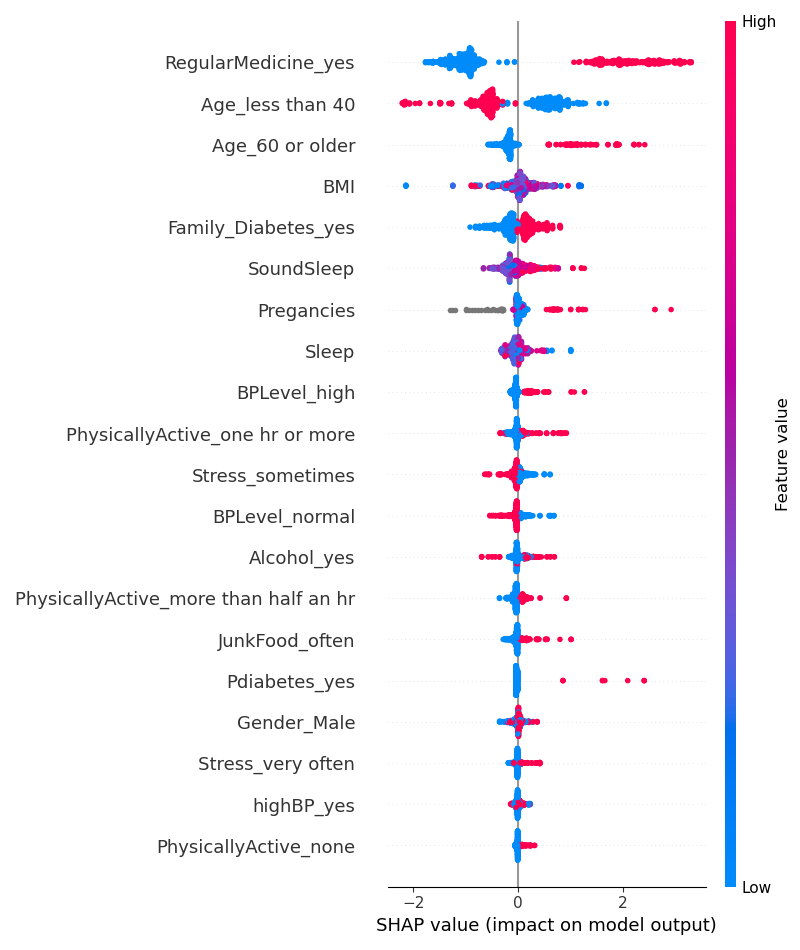
\includegraphics[scale=0.5]{images/shap_lgbm_diabete.png}
\end{figure}

E no final, podemos identificar quais foram os hiperparâmetros com maior impacto em cada um dos modelos e quais foram seus valores.
\begin{table}[H]
\centering
\begin{tabular}{|c|c|c|}
\hline
\textbf{Modelo} & \multicolumn{2}{c|}{\textbf{Hiperparâmetros}} \\
\hline
\textbf{XGBoost} & 'min\_child\_weight': 1 & \\
\hline
\textbf{CatBoost} &'depth': 10 & 'learning\_rate': 0.005585552379158199 \\
\hline
\textbf{LightGBM} &'lambda\_l1': 2.7481689793447196e-06 & learning\_rate': 0.08425779644832665 \\
\hline
\end{tabular}
\caption{Valores finais dos hiperparâmetros com maiores impactos em cada modelo no conjunto de dado de Diabetes.}
\end{table}

Para o XGBoost, o modelo otimizado pelo optuna tem o hiperparâmetro 'min\_child\_weight': 1, e como esse hiperparâmetro é o com maior importância, podemos analisar o seu comportamento ao longo do estudo. 
\begin{figure}[H]
 \caption{Hiperparâmetros \textit{min\_child\_weight} do XGBoost no estudo do Optuna no conjunto de dados de Diabetes.}.
 \label{fig:op:dia:min:xgb}
 \centering
 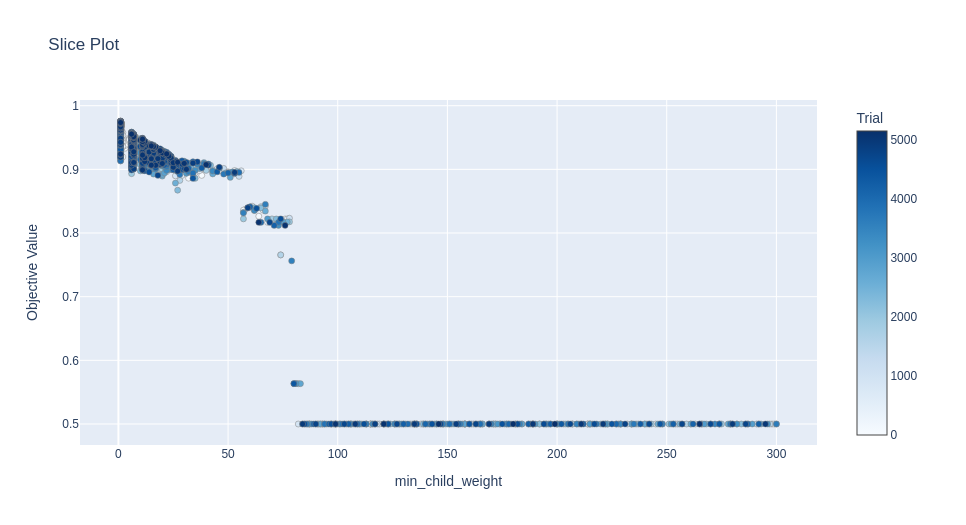
\includegraphics[scale=0.3]{images/optuna_xgboost_min_dia.png}
\end{figure}
Claramente a figura \ref{fig:op:dia:min:xgb} nos mostra que existe uma relação de performance com \textit{min\_child\_weight}: para valores altos do hiperparâmetro a performance cai drasticamente e os melhores valores estão próximos do 0.

Para o CatBoost, o modelo otimizado pelo optuna tem os hiperparâmetros 'depth': 10 e o 'learning\_rate': 0.005585552379158199, e como esses hiperparâmetros são os que possuem as maiores importância no estudo, podemos analisar os seus impactos. 
\begin{figure}[H]
 \caption{Hiperparâmetros \textit{depth} do CatBoost no estudo do Optuna no conjunto de dados de Diabetes.}.
 \label{fig:op:dia:dep:cat}
 \centering
 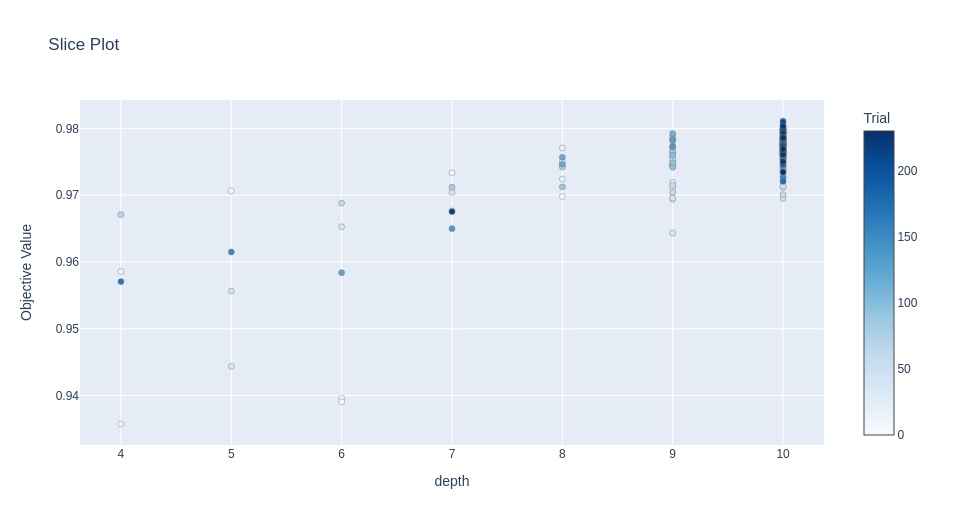
\includegraphics[scale=0.3]{images/optuna_cat_depth_dia.png}
\end{figure}
\begin{figure}[H]
 \caption{Hiperparâmetros \textit{learning\_rate} do CatBoost no estudo do Optuna no conjunto de dados de Diabetes.}.
 \label{fig:op:dia:len:cat}
 \centering
 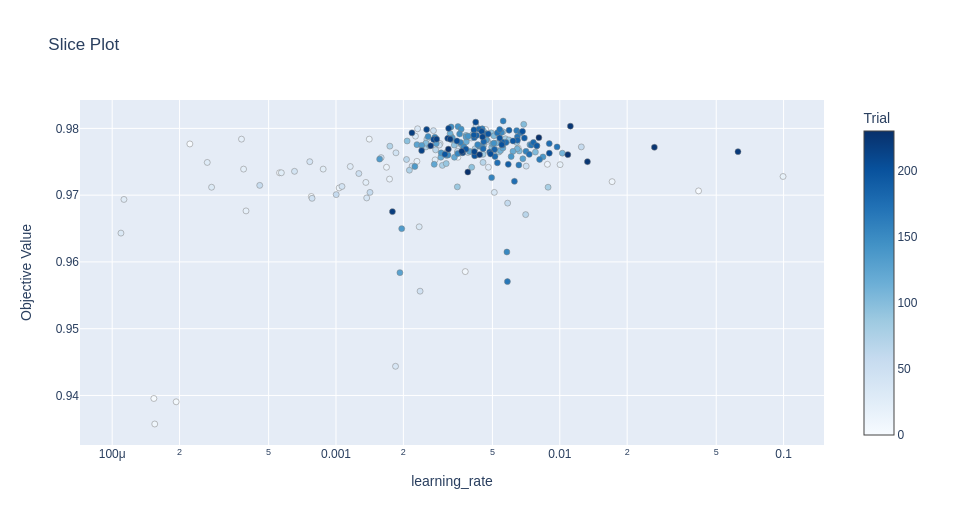
\includegraphics[scale=0.3]{images/optuna_cat_learnig_dia.png}
\end{figure}
A figura \ref{fig:op:dia:dep:cat} nos mostra que existe uma relação de performance com o crescimento do \textit{depth}, com os melhores valores e concentranto no 10. Enquanto que a figura \ref{fig:op:dia:len:cat} o \textit{learning\_rate} tem uma melhor performance na região de 0.001 até 0.01.


No LightGBM, o modelo otimizado pelo optuna tem os hiperparâmetros 'lambda\_l1': 2.7481689793447196e-06 e o learning\_rate': 0.08425779644832665, e como esses hiperparâmetros são os mais importantes no estudo, podemos analisar os seus impactos.

\begin{figure}[H]
 \caption{Hiperparâmetros \textit{lambda\_l1} do LightGBM no estudo do Optuna no conjunto de dados de Diabetes.}.
 \label{fig:op:dia:lamb:lgbm}
 \centering
 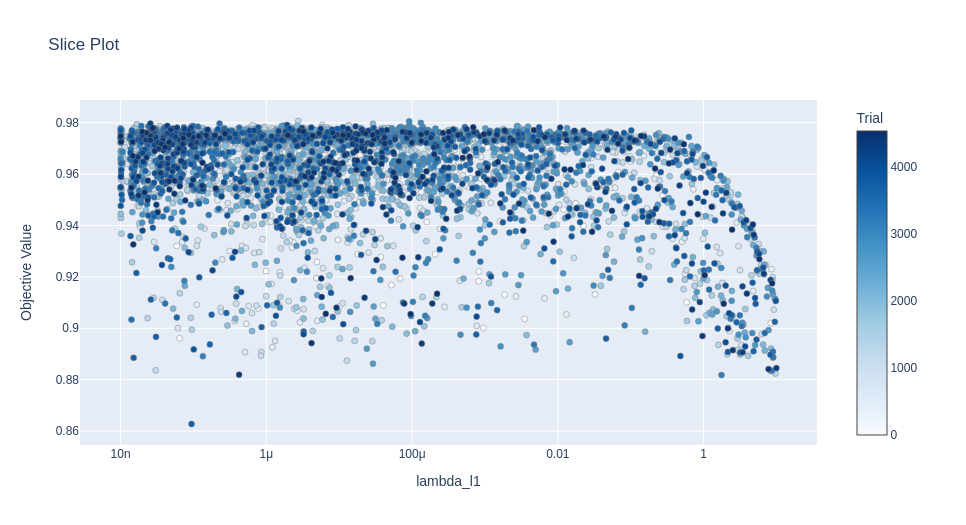
\includegraphics[scale=0.3]{images/optuna_lgbm_lambda_dia.png}
\end{figure}
\begin{figure}[H]
 \caption{Hiperparâmetros \textit{learning\_rate} do LightGBM no estudo do Optuna no conjunto de dados de Diabetes.}.
 \label{fig:op:dia:learn:lgbm}
 \centering
 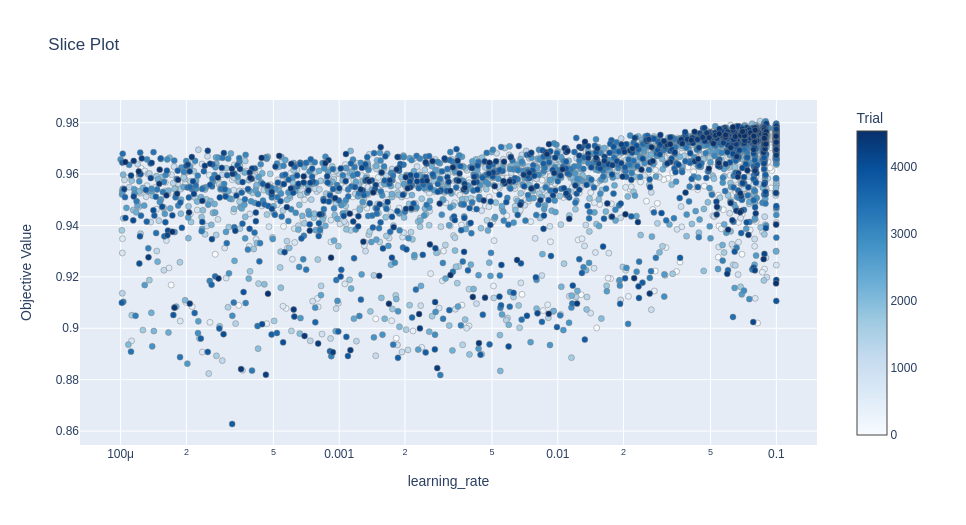
\includegraphics[scale=0.3]{images/optuna_lgbm_learn_dia.png}
\end{figure}
Na figura \ref{fig:op:dia:lamb:lgbm}, podemos perceber que começa uma leve queda na performance a partir de valores \textit{lambda\_l1} maiores que 0.01, ficando mais evidente com valores próximo de 1. E na figura \ref{fig:op:dia:learn:lgbm} existe uma relação de crescimento de performance conforme os valores de \textit{learning\_rate} vão aumentando, ficando claro que a região com maior performance está perto de  \textit{learning\_rate} com o valor de 0.1.

\section{Resultados Finais Insuficiência Cardíaca}
A partir das tabelas \ref{res:car:1} e \ref{res:car:op} podemos calcular a diferença de performance em percentual.

\begin{table}[H]
\centering
\begin{tabular}{|c|c|c|c|}
\hline
	& \textbf{XGBoost} &\textbf{CatBoost} & \textbf{LightGBM} \\
\hline
$\delta_{AUC}$	& 12.51\%&	5.52\%	   &     11.06\% \\
\hline
$\delta_{KS}$	&    16.80\% 	&  -1.77\% &	11.52\%\\
\hline
\end{tabular}
\caption{Aumento final da performance do modelo otimizado pelo Optuna para o conjunto de dados de Insuficiência Cardíaca.}
\end{table}

\begin{figure}[H]
 \caption{SHAP Values para o modelo XGBoost do conjunto de dados de Insuficiência Cardíaca}
 \label{shap:fin:car}
 \centering
 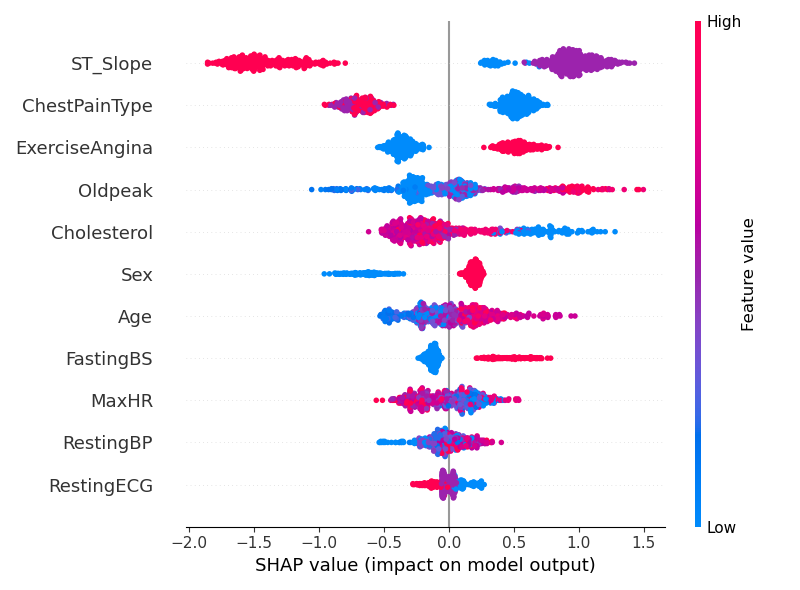
\includegraphics[scale=0.5]{images/shap_lgbm_heart.png}
\end{figure}
E no final, podemos identificar quais foram os hiperparâmetros com maior impacto em cada um dos modelos e quais foram seus valores.
\begin{table}[H]
\centering
\begin{tabular}{|c|c|c|}
\hline
\textbf{Modelo} & \multicolumn{2}{c|}{\textbf{Hiperparâmetros}} \\
\hline
\textbf{XGBoost} & 'min\_child\_weight': 6 & \\
\hline
\textbf{CatBoost} &'learning\_rate': 0.006239961585898258 & 'l2\_leaf\_reg': 9.62802219566606 \\
\hline
\textbf{LightGBM} &'learning\_rate': 0.0765705960307223 & 'min\_data\_in\_leaf': 26 \\
\hline
\end{tabular}
\caption{Valores finais dos hiperparâmetros com maiores impactos em cada modelo no conjunto de dado de Insuficiência Cardíaca.}
\end{table}
Para o XGBoost novamente o \textit{min\_child\_weight} se destacou, mostrando que para valores menores que 50 é onde estão as melhores performances do modelo.
\begin{figure}[H]
 \caption{Hiperparâmetros \textit{min\_child\_weight} do XGBoost no estudo do Optuna no conjunto de dados de Insuficiência Cardíaca.}
 \label{fig:op:heart:min:xgb}
 \centering
 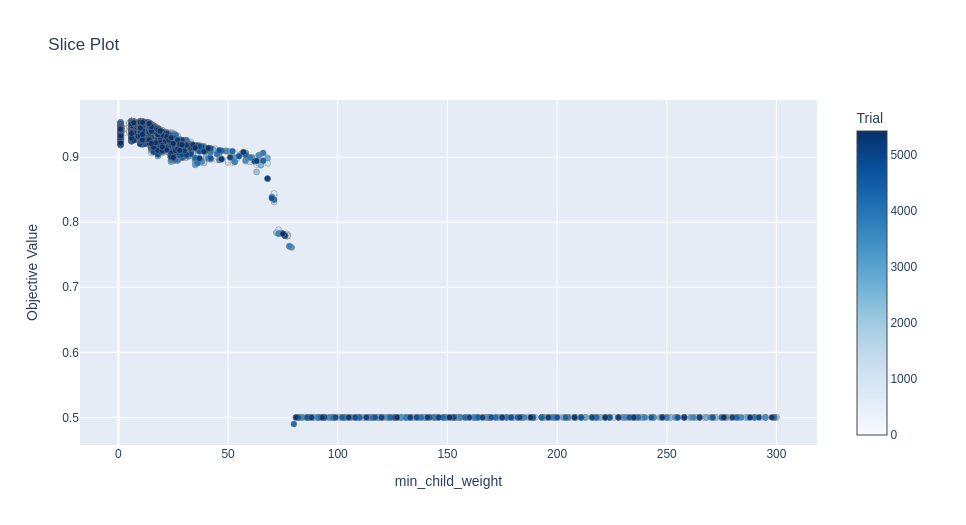
\includegraphics[scale=0.3]{images/optuna_xgboost_min_heart.png}
\end{figure}

Para o CatBoost temos \textit{learning\_rate} e o \textit{l2\_leaf\_reg} com as maiores importâncias no estudo.
\begin{figure}[H]
 \caption{Hiperparâmetros \textit{learning\_rate} do CatBoost no estudo do Optuna no conjunto de dados de Insuficiência Cardíaca.}
 \label{fig:op:heart:learn:cat}
 \centering
 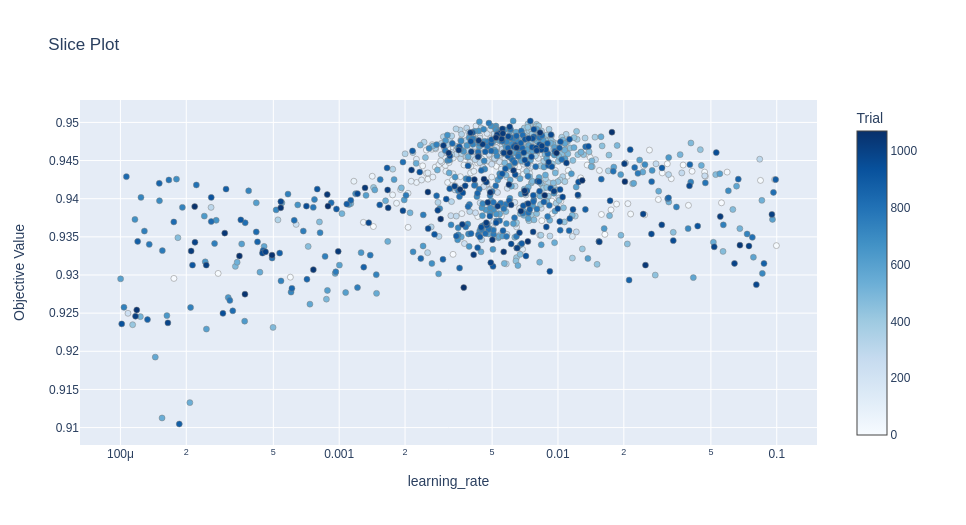
\includegraphics[scale=0.3]{images/optuna_catboost_learning_heart.png}
\end{figure}
\begin{figure}[H]
 \caption{Hiperparâmetros \textit{l2\_leaf\_reg} do CatBoost no estudo do Optuna no conjunto de dados de Insuficiência Cardíaca.}
 \label{fig:op:heart:l2:cat}
 \centering
 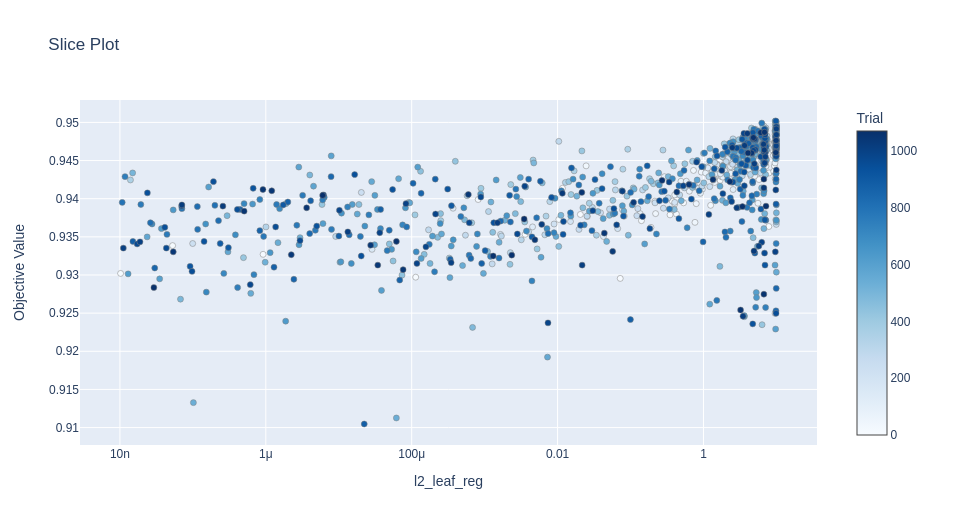
\includegraphics[scale=0.3]{images/optuna_catboost_l2_heart.png}
\end{figure}

Podemos concluir que, para o \textit{learning\_rate}, a região com a melhor performance está entre 0.005 e 0.01 e para \textit{l2\_leaf\_reg} existe uma relação de aumento de performance com o aumento desse hiperparâmetro, sendo a região com maior performance com \textit{l2\_leaf\_reg} acima de 1.

Para o LightLGBM temos o \textit{learning\_rate} e o \textit{min\_data\_in\_leaf} que somados representam 70\% da importancia do estudo.
\begin{figure}[H]
 \caption{Hiperparâmetros \textit{learning\_rate}  do LightGBM no estudo do Optuna no conjunto de dados de Insuficiência Cardíaca.}.
 \label{fig:op:heart:learn:lgbm}
 \centering
 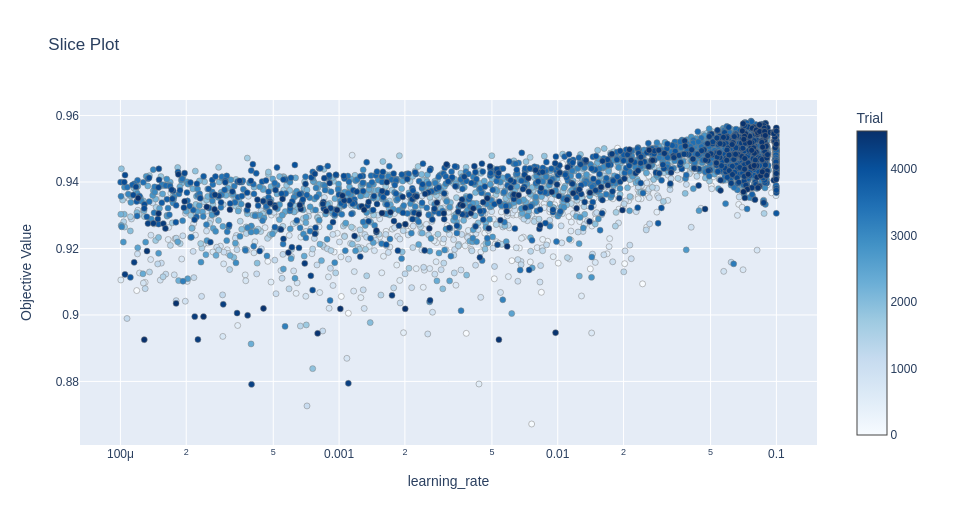
\includegraphics[scale=0.3]{images/optuna_lgbm_learning_heart.png}
\end{figure}
\begin{figure}[H]
 \caption{Hiperparâmetros \textit{min\_data\_in\_leaf} do LightGBM no estudo do Optuna no conjunto de dados de Insuficiência Cardíaca.}
 \label{fig:op:heart:min:lgbm}
 \centering
 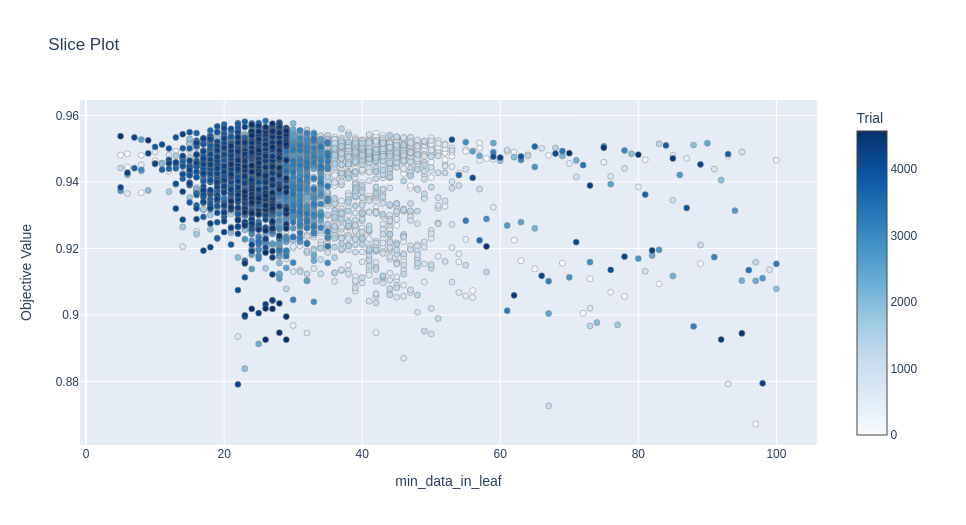
\includegraphics[scale=0.3]{images/optuna_lgbm_min_heart.png}
\end{figure}

Conforme o \textit{learning\_rate} vai aumentado, a perfomance do estudo também aumenta sendo que o melhor valor está próximo de \textit{learning\_rate} com 0.1. E para \textit{min\_data\_in\_leaf} conseguimos perceber que valores abaixo de 80 já temos uma boa performance.
\section{Resultados Finais Insuficiência Renal}
A partir das tabelas \ref{res:ren:1} e \ref{res:ren:op} podemos calcular a diferença de performance em percentual.

\begin{table}[H]
\centering
\begin{tabular}{|c|c|c|c|}
\hline
	& \textbf{XGBoost} &\textbf{CatBoost} & \textbf{LightGBM} \\
\hline
$\delta_{AUC}$	& 31.76\%&	23.53\%	   &     21.57\% \\
\hline
$\delta_{KS}$	& 140.00\%     	&  56.26\% &	59.37\%\\
\hline
\end{tabular}
\caption{Aumento final da performance do modelo otimizado pelo Optuna para o conjunto de dados de Insuficiência Renal.}
\end{table}

\begin{figure}[H]
 \caption{SHAP Values para o modelo CatBoost do conjunto de dados de Insuficiência Renal}
 \label{shap:fin:ren}
 \centering
 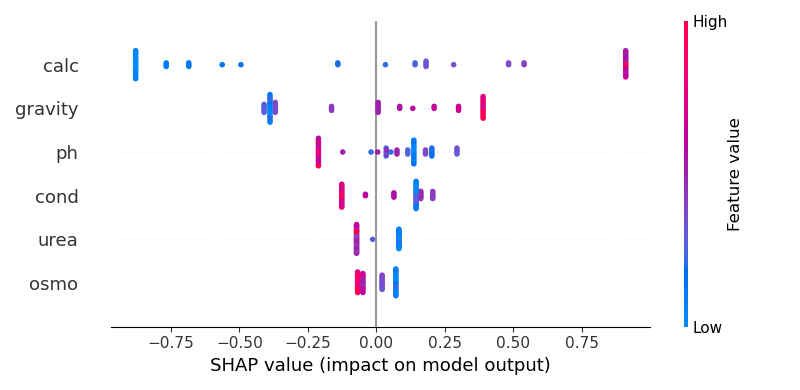
\includegraphics[scale=0.5]{images/shap_lgbm_kidney.png}
\end{figure}
E no final, podemos identificar quais foram os hiperparâmetros com maior impacto em cada um dos modelos e quais foram seus valores.
\begin{table}[H]
\centering
\begin{tabular}{|c|c|c|}
\hline
\textbf{Modelo} & \multicolumn{2}{c|}{\textbf{Hiperparâmetros}} \\
\hline
\textbf{XGBoost} & 'min\_child\_weight': 4 & \\
\hline
\textbf{CatBoost} &'depth': 5 & 'learning\_rate': 0.07537894328903638 \\
\hline
\textbf{LightGBM} & 'min\_data\_in\_leaf': 7 &  \\
\hline
\end{tabular}
\caption{Valores finais dos hiperparâmetros com maiores impactos em cada modelo no conjunto de dado de Insuficiência Renal.}
\end{table}

Para o XGBoost o hiperparâmetros com maior impacto foi novamente o \textit{min\_child\_weight}
\begin{figure}[H]
 \caption{Hiperparâmetros \textit{min\_child\_weight} do XGBoost no estudo do Optuna no conjunto de dados de Insuficiência Renal.}
 \label{fig:op:kind:min:xgb}
 \centering
 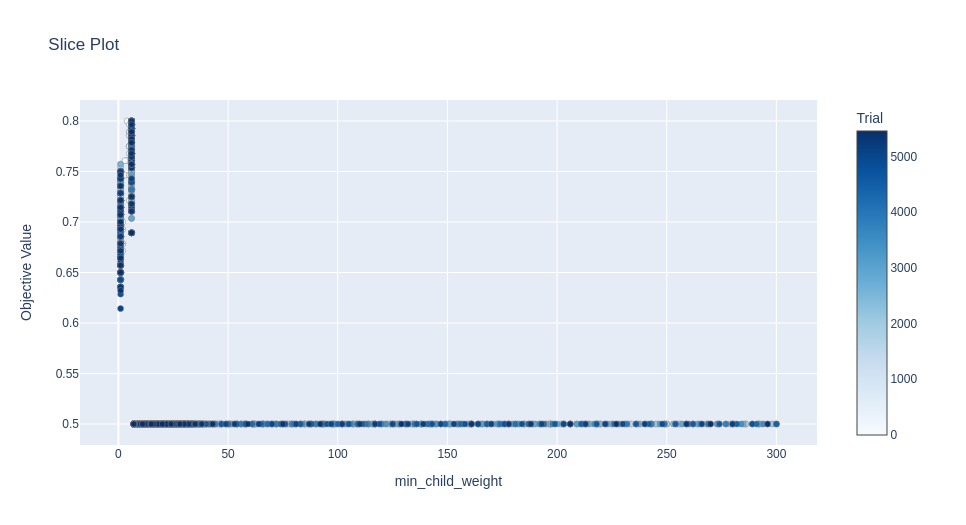
\includegraphics[scale=0.3]{images/optuna_min_xgboost_kindey.png}
\end{figure}
E podemos perceber que a performance fica satisfatória para valores de \textit{min\_child\_weight} abaixo de 10.

Para o CatBoost os hiperparâmetros que representaram quase 80\% da importância foram o \textit{depth} e o \textit{learning\_rate}.
\begin{figure}[H]
 \caption{Hiperparâmetros \textit{depth} do CatBoost no estudo do Optuna no conjunto de dados de Insuficiência Renal.}.
 \label{fig:op:kind:depth:cat}
 \centering
 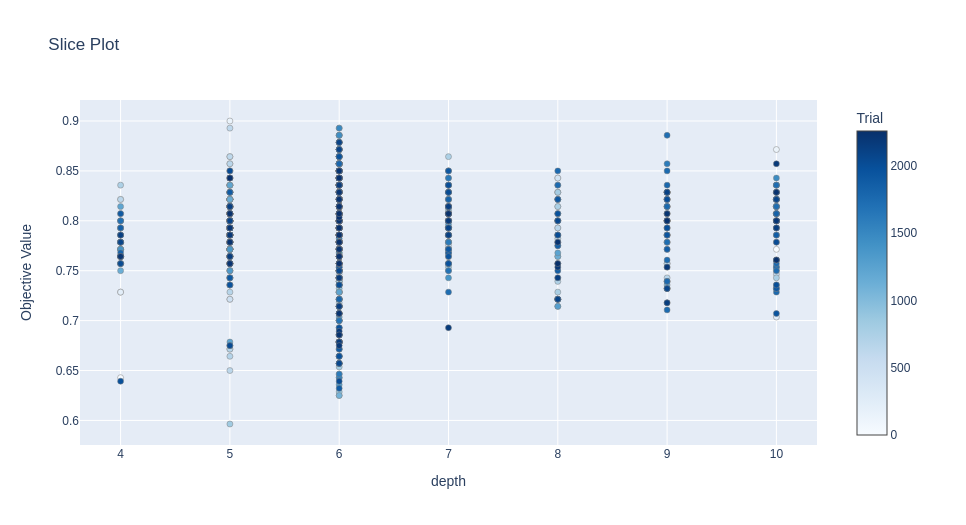
\includegraphics[scale=0.3]{images/opatuna_catboost_depth_kindey.png}
\end{figure}
\begin{figure}[H]
 \caption{Hiperparâmetros \textit{learning\_rate} do CatBoost no estudo do Optuna no conjunto de dados de Insuficiência Renal.}
 \label{fig:op:kind:learn:cat}
 \centering
 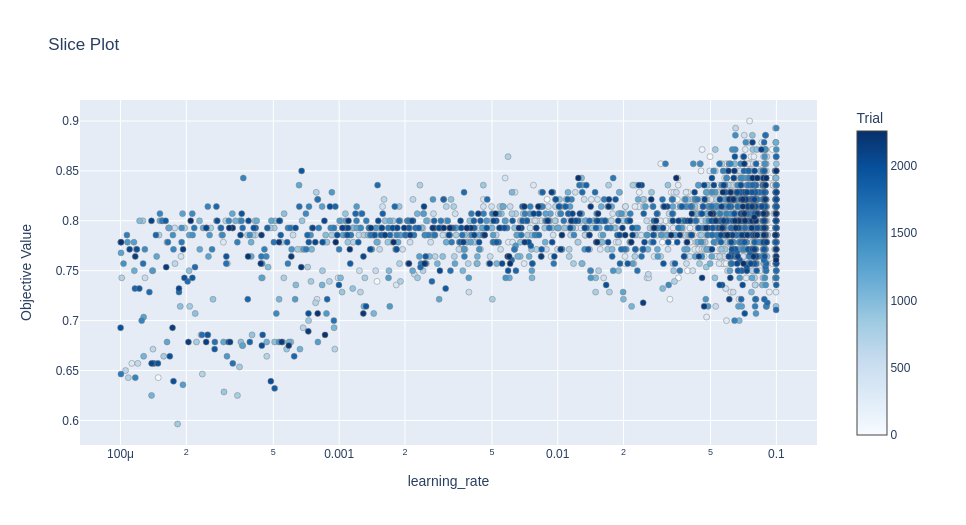
\includegraphics[scale=0.3]{images/optuna_learning_rate-catboost_kindey.png}
\end{figure}
Pela figura \ref{fig:op:kind:depth:cat} percebe-se que os melhores valores se concentram em 5, 6 e 9 para \textit{depth}. E na figura \ref{fig:op:kind:learn:cat} os maiores valores de \textit{learning\_rate}, próximo a 0.1, são os que apresentaram a melhor performance.

Para o LightGBM o \textit{min\_data\_in\_leaf} apresentou 95\% da importância.
\begin{figure}[H]
 \caption{Hiperparâmetros do LightGBM no estudo do Optuna no conjunto de dados de Insuficiência Renal.}
 \label{fig:op:kind:min:lgbm}
 \centering
 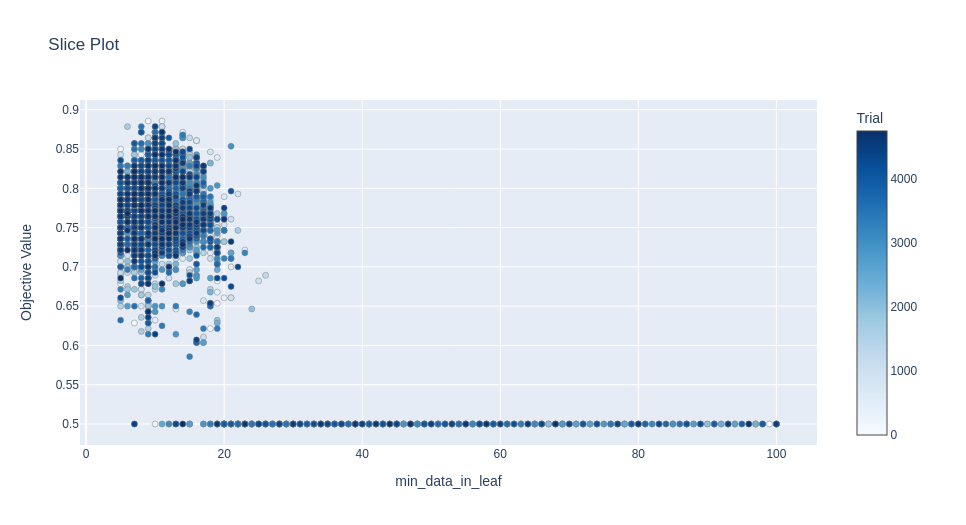
\includegraphics[scale=0.3]{images/optuna_min_lgbm_kindey.png}
\end{figure}
Sendo que valores abaixo de 20 obtiverem as melhores performances.
\section{Resultados Finais Carcinoma de Mama}
A partir das tabelas \ref{res:can:1} e \ref{res:can:op}, podemos calcular a diferença de performance em percentual.

\begin{table}[H]
\centering
\begin{tabular}{|c|c|c|c|}
\hline
	& \textbf{XGBoost} &\textbf{CatBoost} & \textbf{LightGBM} \\
\hline
$\delta_{AUC}$	& 1.97\%&	2.85\%	   &     5.75\% \\
\hline
$\delta_{KS}$	& 2.62\%    	&  3.37\% &	10.55\%\\
\hline
\end{tabular}
\caption{Aumento final da performance do modelo otimizado pelo Optuna para o conjunto de dados de Carcinoma de Mama.}
\end{table}

\begin{figure}[H]
 \caption{SHAP Values para o modelo LightGBM do conjunto de dados de Carcinoma de Mama}
 \label{shap:fin:canc}
 \centering
 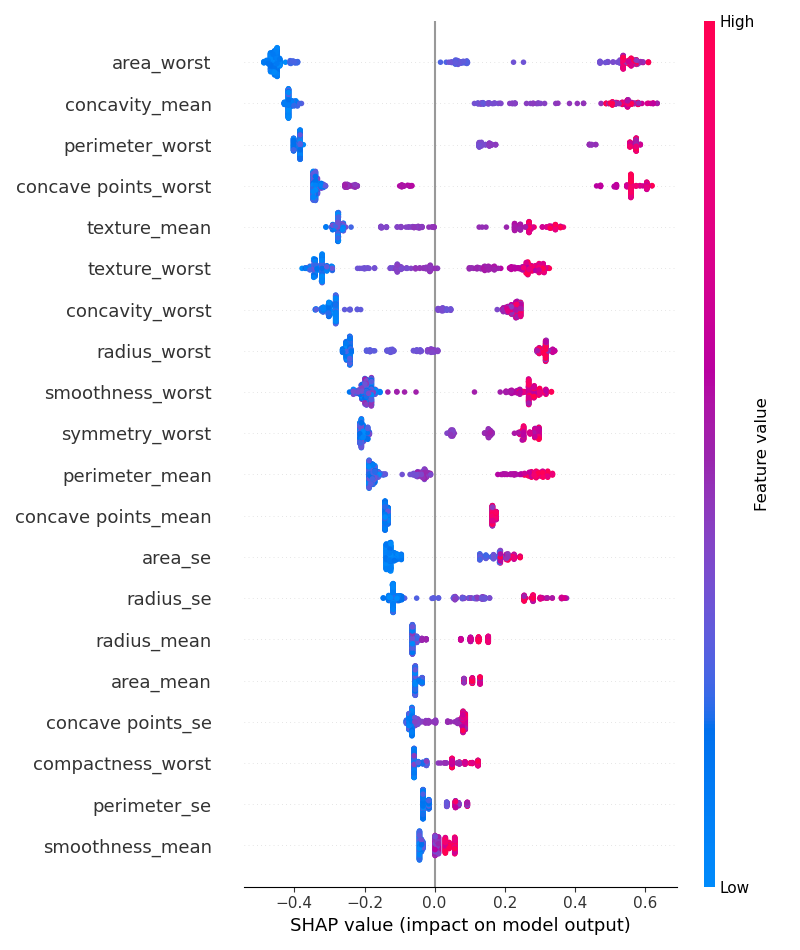
\includegraphics[scale=0.5]{images/shap_cancer.png}
\end{figure}

\begin{table}[H]
\centering
\begin{tabular}{|c|c|c|}
\hline
\textbf{Modelo} & \multicolumn{2}{c|}{\textbf{Hiperparâmetros}} \\
\hline
\textbf{XGBoost} & 'min\_child\_weight': 15 & \\
\hline
\textbf{CatBoost} &'random\_strength': 5.267279748486068 & 'learning\_rate': 0.014693012954604871\\
\hline
\textbf{LightGBM} & 'min\_data\_in\_leaf': 66 & 'learning\_rate': 0.07615521372640538 \\
\hline
\end{tabular}
\caption{Valores finais dos hiperparâmetros com maiores impactos em cada modelo no conjunto de dados de Carcinoma de Mama.}
\end{table}

Para o XGBoost o hiperparâmetro \textit{min\_child\_weight} teve a maior importância.
\begin{figure}[H]
 \caption{Hiperparâmetro \textit{min\_child\_weight} do XGBoost no estudo do Optuna no conjunto de dados de Carcinoma de Mama.}
 \label{fig:op:cancer:min:xgb}
 \centering
 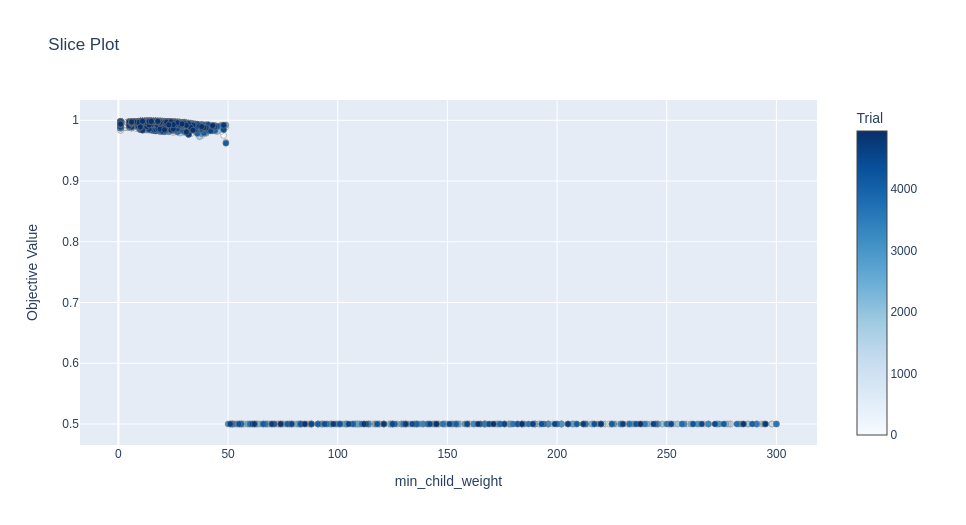
\includegraphics[scale=0.3]{images/optuna_xgboost_min_cancer.png}
\end{figure}
Então para valores abaixo de 50 o modelo teve as melhores performances.

Para o CatBoost os hiperparâmetros \textit{random\_strength} e o \textit{learning\_rate} representam 87\% da importância.
\begin{figure}[H]
 \caption{Hiperparâmetros \textit{random\_strength} do CatBoost no estudo do Optuna no conjunto de dados de Carcinoma de Mama.}
 \label{fig:op:cancer:rad:cat}
 \centering
 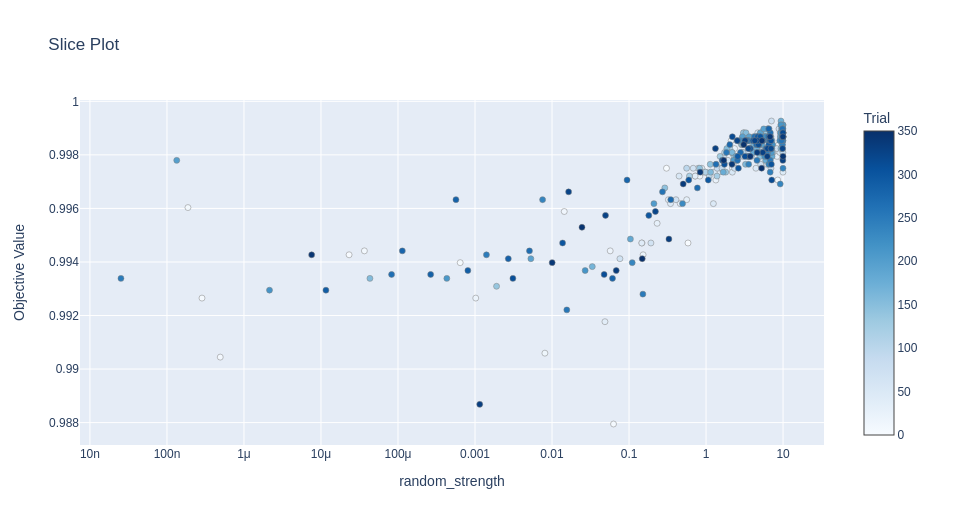
\includegraphics[scale=0.3]{images/optuna_catboost_random_cancer.png}
\end{figure}
\begin{figure}[H]
 \caption{Hiperparâmetros \textit{learning\_rate} do CatBoost no estudo do Optuna no conjunto de dados de Carcinoma de Mama.}
 \label{fig:op:cancer:len:cat}
 \centering
 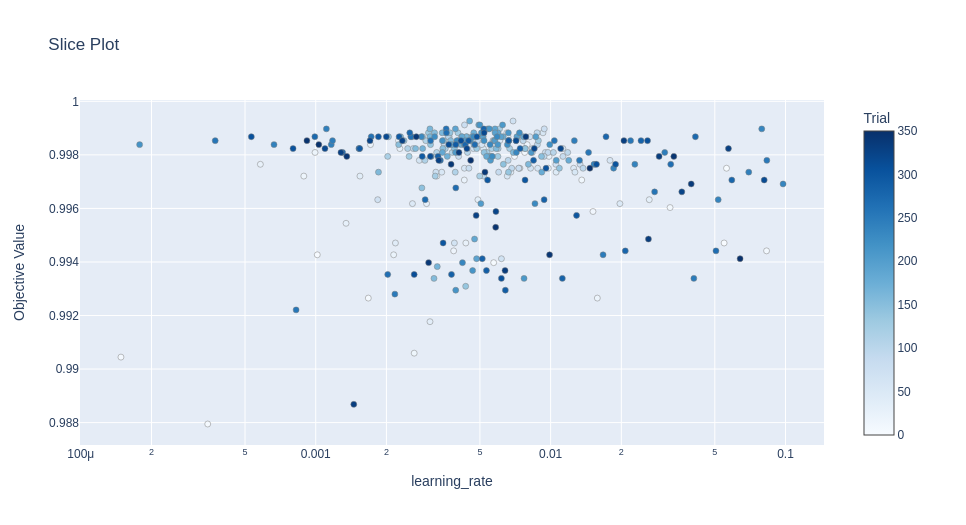
\includegraphics[scale=0.3]{images/optuna_catboost_learning_cancer.png}
\end{figure}
Pela figura \ref{fig:op:cancer:rad:cat}, quanto maior o \textit{random\_strength} melhor a perfomance do modelo, sendo a região entre 5 e 10 ideal. E na figura \ref{fig:op:cancer:len:cat} podemos perceber que o \textit{learning\_rate} entre 0.001 até 0.1 teve bons resultados, sendo essa uma boa região para escolher.

Para o LightGBM os hiperparâmetros \textit{min\_data\_in\_leaf} e \textit{learning\_rate}  representaram 90\% da importância.
\begin{figure}[H]
 \caption{Hiperparâmetros \textit{min\_data\_in\_leaf} do LightGBM no estudo do Optuna no conjunto de dados de Carcinoma de Mama.}
 \label{fig:op:cancer:min:lgbm}
 \centering
 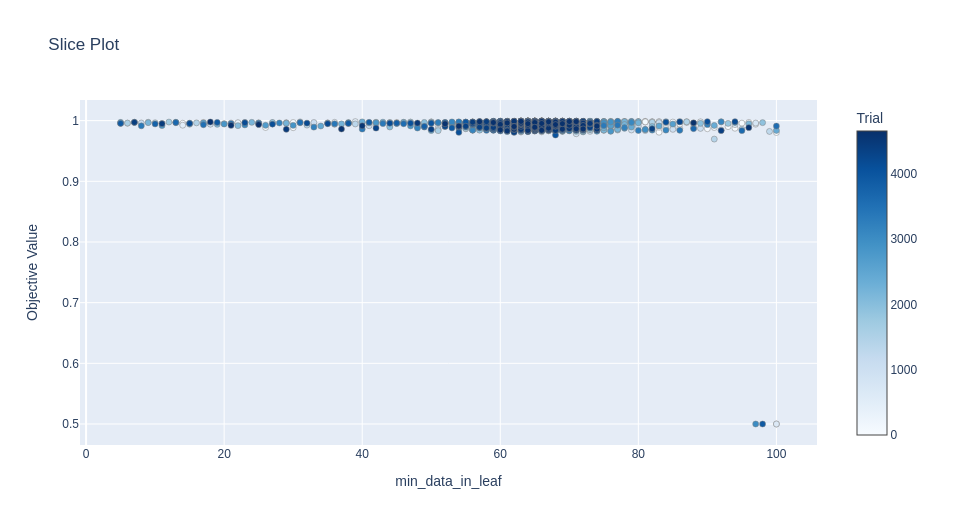
\includegraphics[scale=0.3]{images/optuna_lgbm_min_cancer.png}
\end{figure}
\begin{figure}[H]
 \caption{Hiperparâmetros \textit{learning\_rate} do LightGBM no estudo do Optuna no conjunto de dados de Carcinoma de Mama.}
 \label{fig:op:cancer:learn:lgbm}
 \centering
 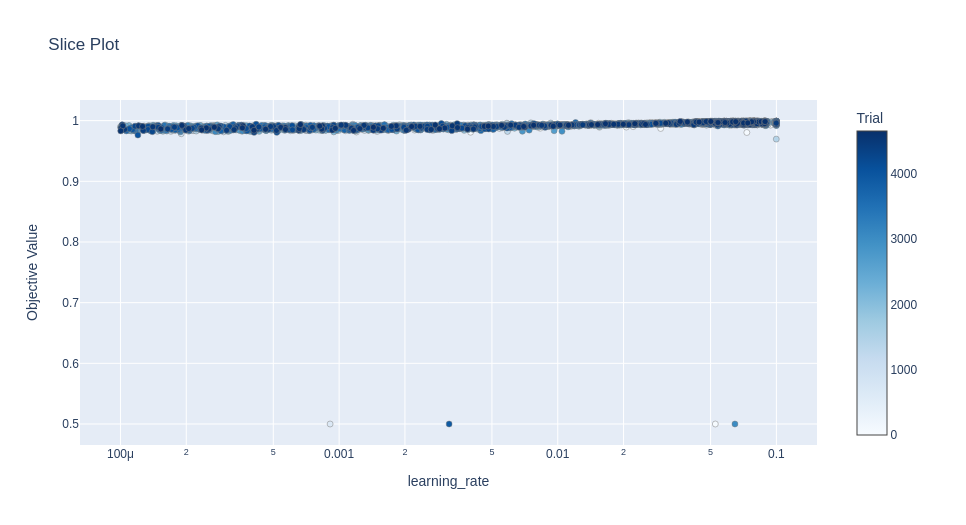
\includegraphics[scale=0.3]{images/optuna_lgbm_learning_cancer.png}
\end{figure}
Na figura \ref{fig:op:cancer:min:lgbm} podemos perceber que não é possível concluir uma região ótima para o \textit{min\_data\_in\_leaf} nem para o \textit{learning\_rate}. Isso aconteceu pelo fato do modelo já ter conseguido ótimas performances iniciais e talvez o espaço dos Hiperparâmetros do LightGBM devesse ter sido divido em mais intervalos.